\documentclass[11pt]{article}
\usepackage[textwidth=18.0cm, textheight=23.0cm, top=2.0cm]{geometry}
\usepackage{pst-all}
\usepackage{amssymb}
\usepackage{tikz}
\usepackage{underscore}\begin{document}
\pagestyle{empty}


ClassName: \underline{\textbf{Class_07.2bp-27}}
\par
BinSize: \underline{\textbf{100 × 100}}
\par
ReduceSize: \underline{\textbf{100 × 100}}
\par
TypeNum: \underline{\textbf{59}}
\par
Num: \underline{\textbf{60}}
\par
OutS: \underline{\textbf{170000}}
\par
InS: \underline{\textbf{145305}}
\par
Rate: \underline{\textbf{0.855}}
\par
UB: \underline{\textbf{17}}
\par
LB0: \underline{\textbf{17}}
\par
LB: \underline{\textbf{17}}
\par
LBWithCut: \underline{\textbf{17}}
\par
NodeCut: \underline{\textbf{0}}
\par
ExtendedNodeCnt: \underline{\textbf{1}}
\par
GenNodeCnt: \underline{\textbf{1}}
\par
PrimalNode: \underline{\textbf{0}}
\par
ColumnCount: \underline{\textbf{17}}
\par
TotalCutCount: \underline{\textbf{0}}
\par
RootCutCount: \underline{\textbf{0}}
\par
LPSolverCnt: \underline{\textbf{1}}
\par
PricingSolverCnt: \underline{\textbf{0}}
\par
BranchAndBoundNum: \underline{\textbf{1}}
\par
isOpt: \underline{\textbf{true}}
\par
TimeOnInitSolution: \underline{\textbf{600.000 s}}
\par
TimeOnPrimal: \underline{\textbf{0.000 s}}
\par
TimeOnPricing: \underline{\textbf{0.000 s}}
\par
TimeOnRmp: \underline{\textbf{0.063 s}}
\par
TotalTime: \underline{\textbf{600.313 s}}
\par
\newpage


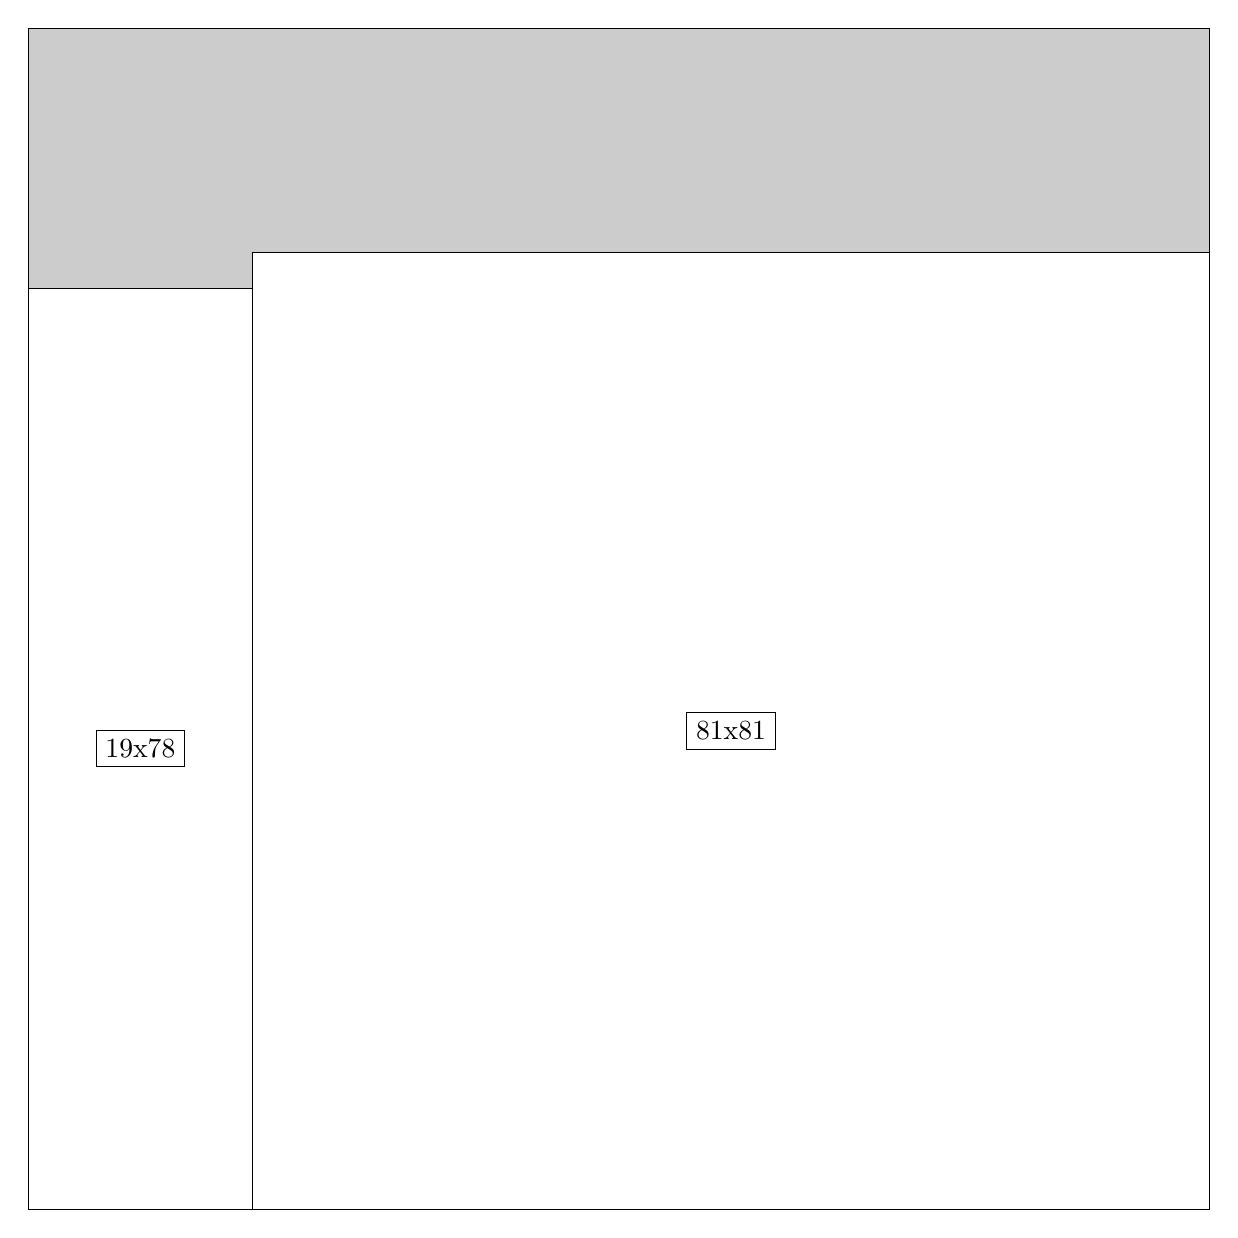
\begin{tikzpicture}[shorten >=1pt,scale=1.0,every node/.style={scale=1.0},->]
\tikzstyle{vertex}=[circle,fill=black!25,minimum size=14pt,inner sep=0pt]
\filldraw[fill=gray!40!white, draw=black] (0,0) rectangle (15.0,15.0);
\foreach \name/\x/\y/\w/\h in {81x81/2.85/0.0/12.15/12.15,19x78/0.0/0.0/2.85/11.7}
\filldraw[fill=white!40!white, draw=black] (\x,\y) rectangle node[draw] (\name) {\name} ++(\w,\h);
\end{tikzpicture}


w =81 , h =81 , x =19 , y =0 , v =6561
\par
w =19 , h =78 , x =0 , y =0 , v =1482
\par
\newpage


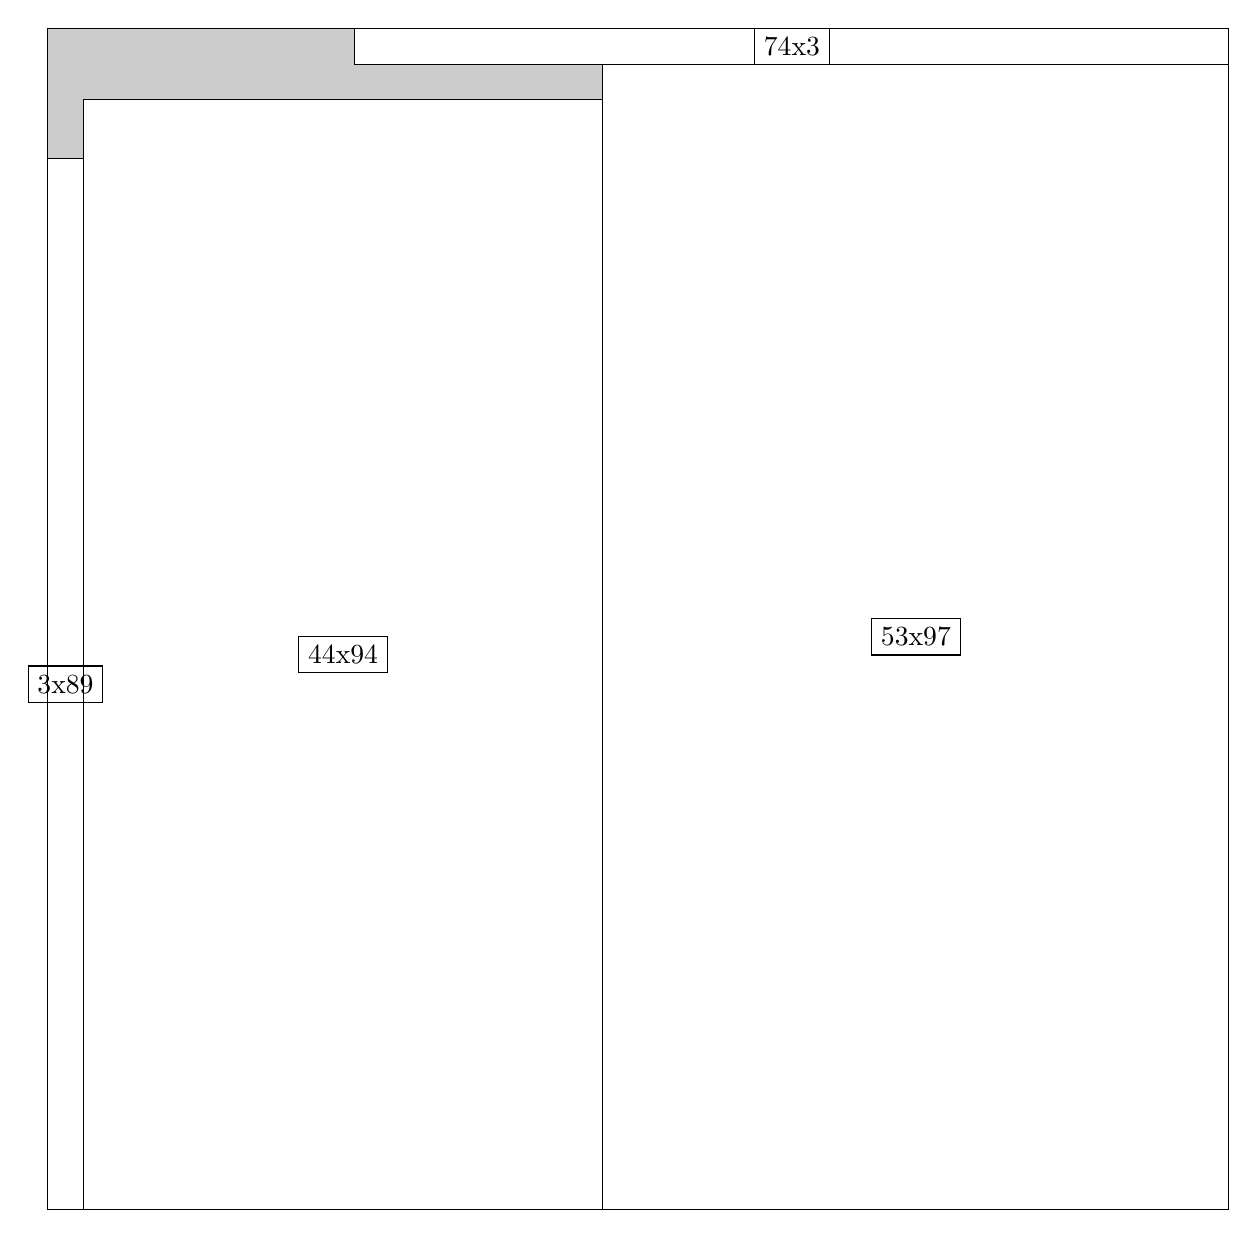
\begin{tikzpicture}[shorten >=1pt,scale=1.0,every node/.style={scale=1.0},->]
\tikzstyle{vertex}=[circle,fill=black!25,minimum size=14pt,inner sep=0pt]
\filldraw[fill=gray!40!white, draw=black] (0,0) rectangle (15.0,15.0);
\foreach \name/\x/\y/\w/\h in {53x97/7.05/0.0/7.949999999999999/14.549999999999999,44x94/0.44999999999999996/0.0/6.6/14.1,3x89/0.0/0.0/0.44999999999999996/13.35,74x3/3.9/14.549999999999999/11.1/0.44999999999999996}
\filldraw[fill=white!40!white, draw=black] (\x,\y) rectangle node[draw] (\name) {\name} ++(\w,\h);
\end{tikzpicture}


w =53 , h =97 , x =47 , y =0 , v =5141
\par
w =44 , h =94 , x =3 , y =0 , v =4136
\par
w =3 , h =89 , x =0 , y =0 , v =267
\par
w =74 , h =3 , x =26 , y =97 , v =222
\par
\newpage


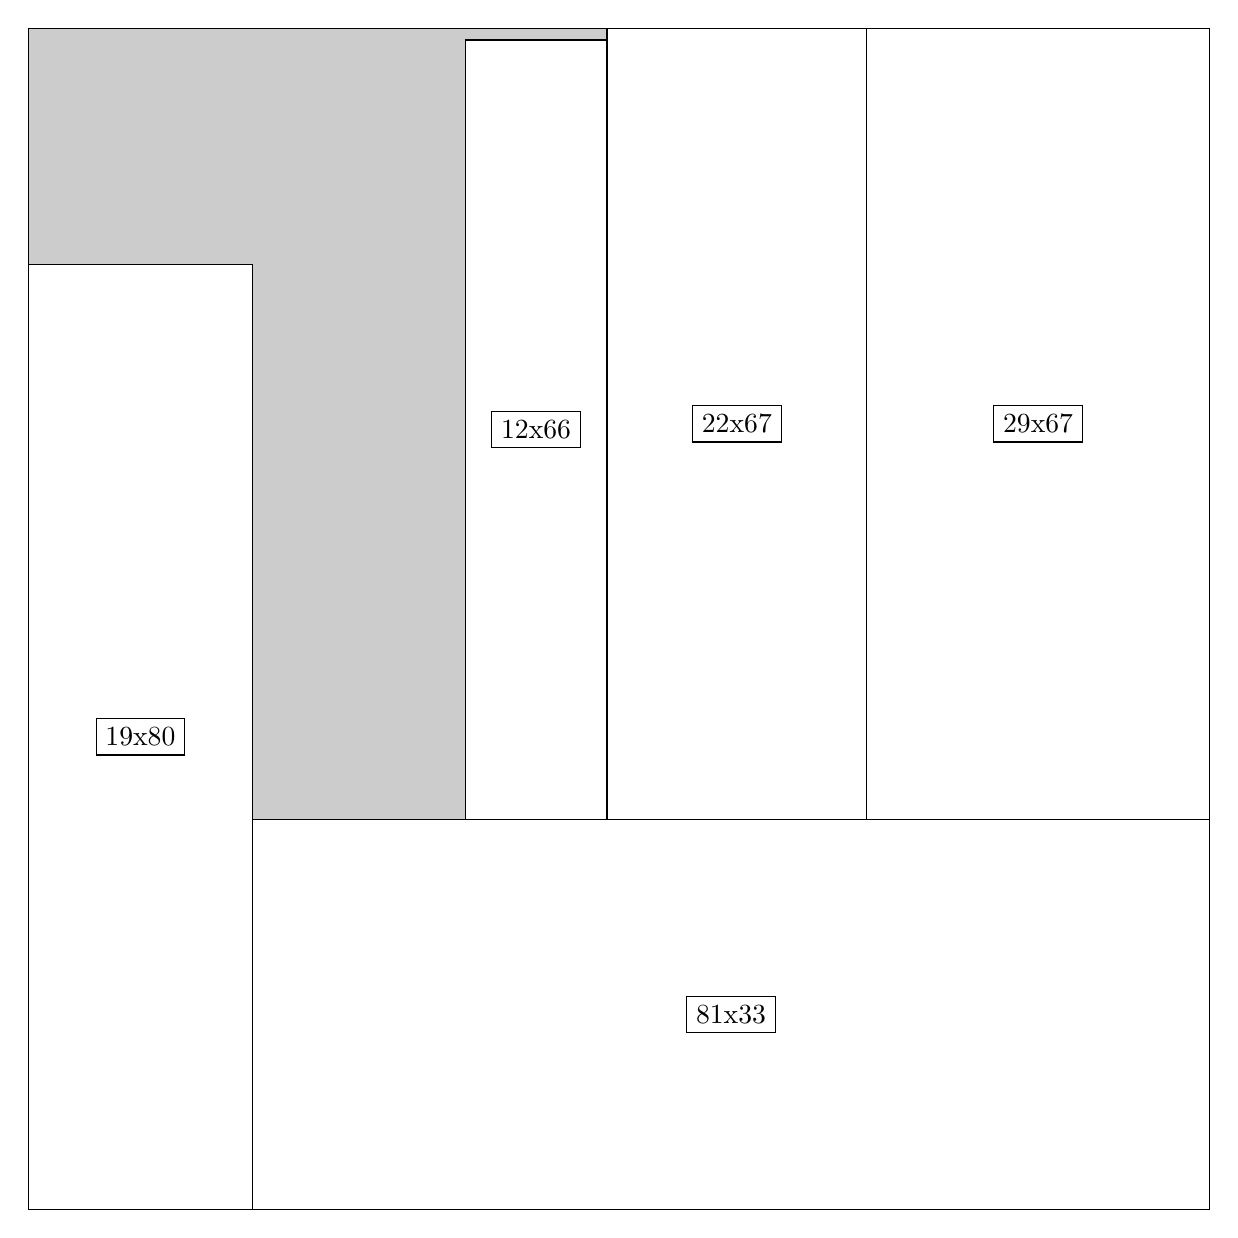
\begin{tikzpicture}[shorten >=1pt,scale=1.0,every node/.style={scale=1.0},->]
\tikzstyle{vertex}=[circle,fill=black!25,minimum size=14pt,inner sep=0pt]
\filldraw[fill=gray!40!white, draw=black] (0,0) rectangle (15.0,15.0);
\foreach \name/\x/\y/\w/\h in {81x33/2.85/0.0/12.15/4.95,29x67/10.65/4.95/4.35/10.049999999999999,22x67/7.35/4.95/3.3/10.049999999999999,12x66/5.55/4.95/1.7999999999999998/9.9,19x80/0.0/0.0/2.85/12.0}
\filldraw[fill=white!40!white, draw=black] (\x,\y) rectangle node[draw] (\name) {\name} ++(\w,\h);
\end{tikzpicture}


w =81 , h =33 , x =19 , y =0 , v =2673
\par
w =29 , h =67 , x =71 , y =33 , v =1943
\par
w =22 , h =67 , x =49 , y =33 , v =1474
\par
w =12 , h =66 , x =37 , y =33 , v =792
\par
w =19 , h =80 , x =0 , y =0 , v =1520
\par
\newpage


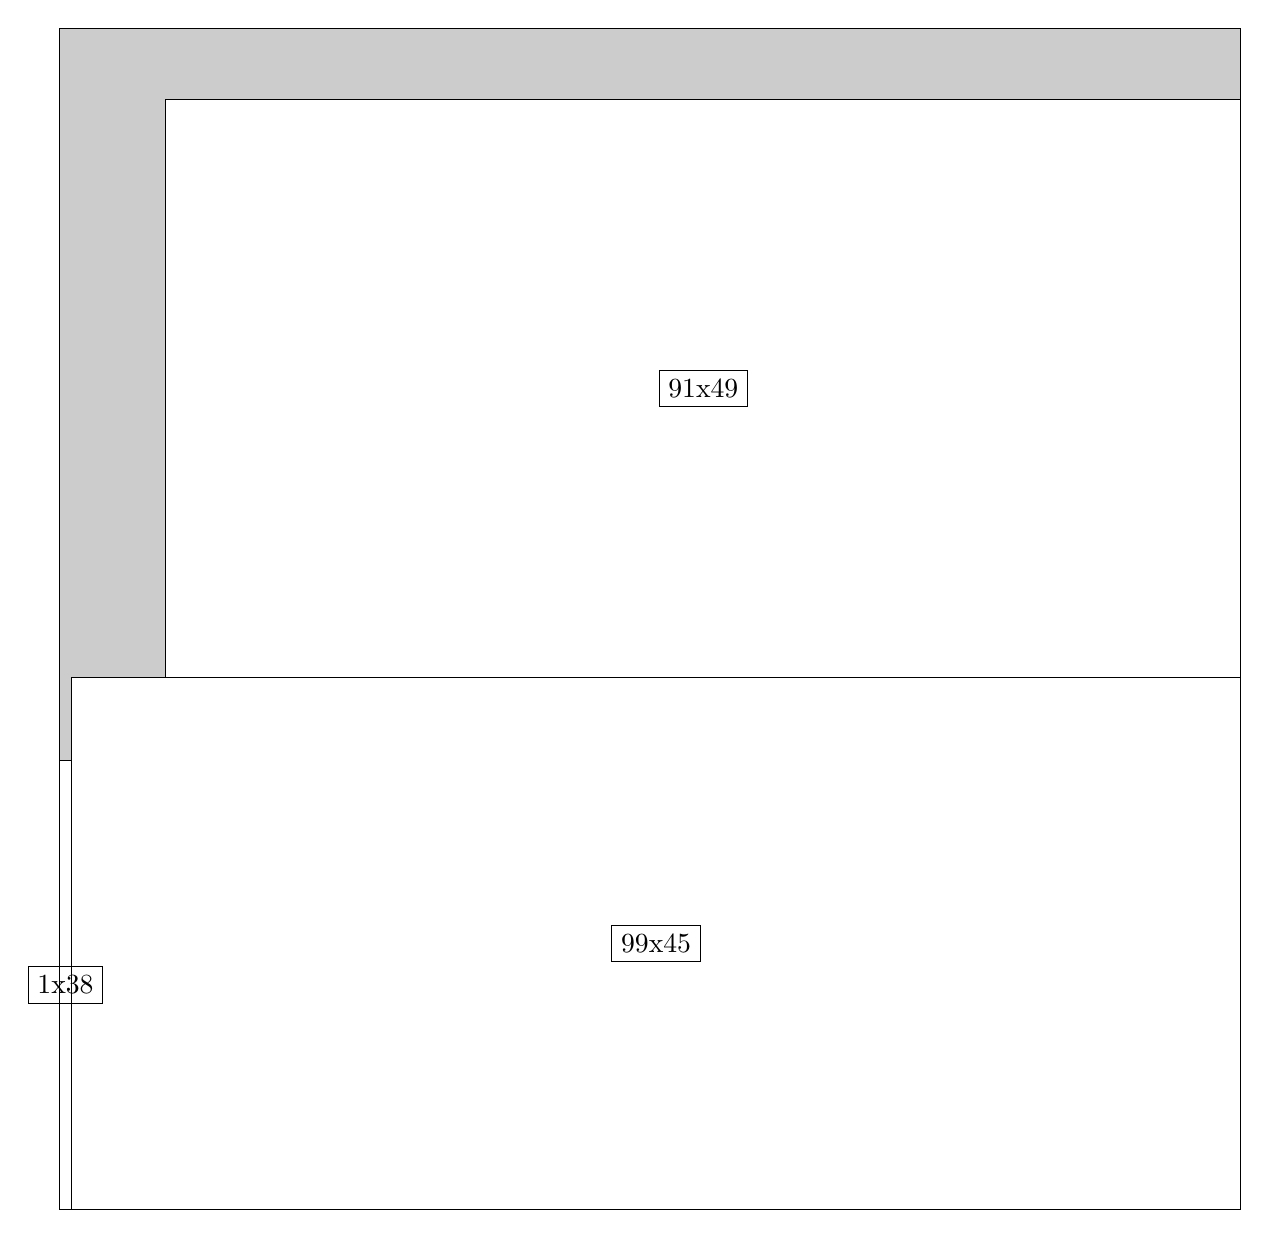
\begin{tikzpicture}[shorten >=1pt,scale=1.0,every node/.style={scale=1.0},->]
\tikzstyle{vertex}=[circle,fill=black!25,minimum size=14pt,inner sep=0pt]
\filldraw[fill=gray!40!white, draw=black] (0,0) rectangle (15.0,15.0);
\foreach \name/\x/\y/\w/\h in {99x45/0.15/0.0/14.85/6.75,1x38/0.0/0.0/0.15/5.7,91x49/1.3499999999999999/6.75/13.65/7.35}
\filldraw[fill=white!40!white, draw=black] (\x,\y) rectangle node[draw] (\name) {\name} ++(\w,\h);
\end{tikzpicture}


w =99 , h =45 , x =1 , y =0 , v =4455
\par
w =1 , h =38 , x =0 , y =0 , v =38
\par
w =91 , h =49 , x =9 , y =45 , v =4459
\par
\newpage


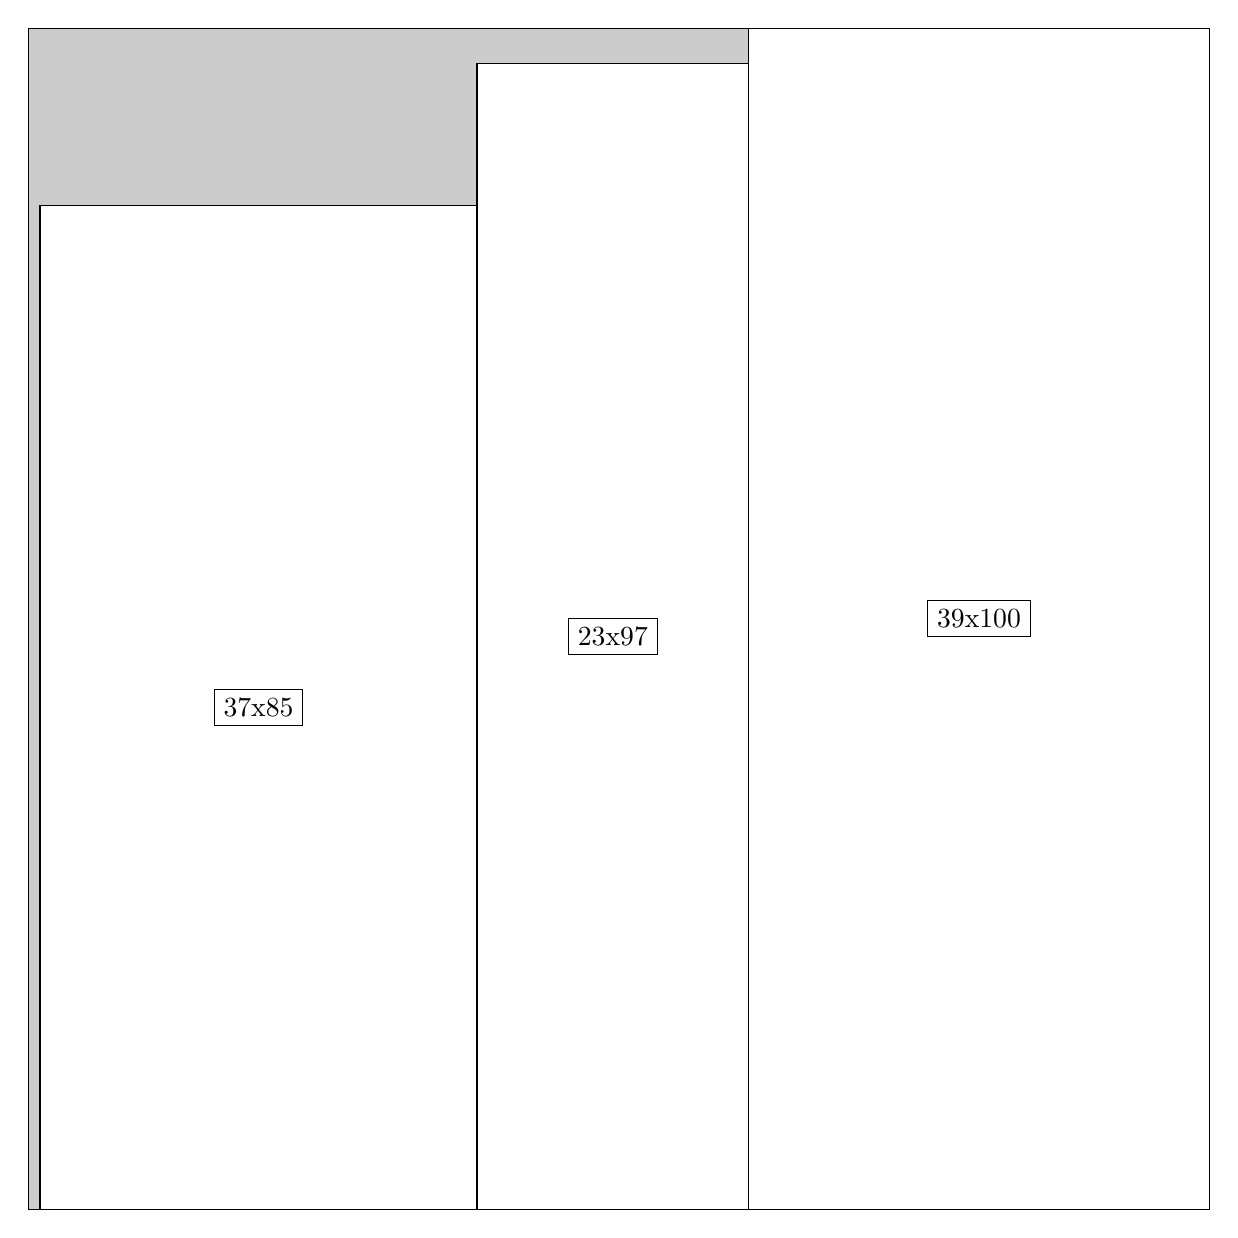
\begin{tikzpicture}[shorten >=1pt,scale=1.0,every node/.style={scale=1.0},->]
\tikzstyle{vertex}=[circle,fill=black!25,minimum size=14pt,inner sep=0pt]
\filldraw[fill=gray!40!white, draw=black] (0,0) rectangle (15.0,15.0);
\foreach \name/\x/\y/\w/\h in {39x100/9.15/0.0/5.85/15.0,23x97/5.7/0.0/3.4499999999999997/14.549999999999999,37x85/0.15/0.0/5.55/12.75}
\filldraw[fill=white!40!white, draw=black] (\x,\y) rectangle node[draw] (\name) {\name} ++(\w,\h);
\end{tikzpicture}


w =39 , h =100 , x =61 , y =0 , v =3900
\par
w =23 , h =97 , x =38 , y =0 , v =2231
\par
w =37 , h =85 , x =1 , y =0 , v =3145
\par
\newpage


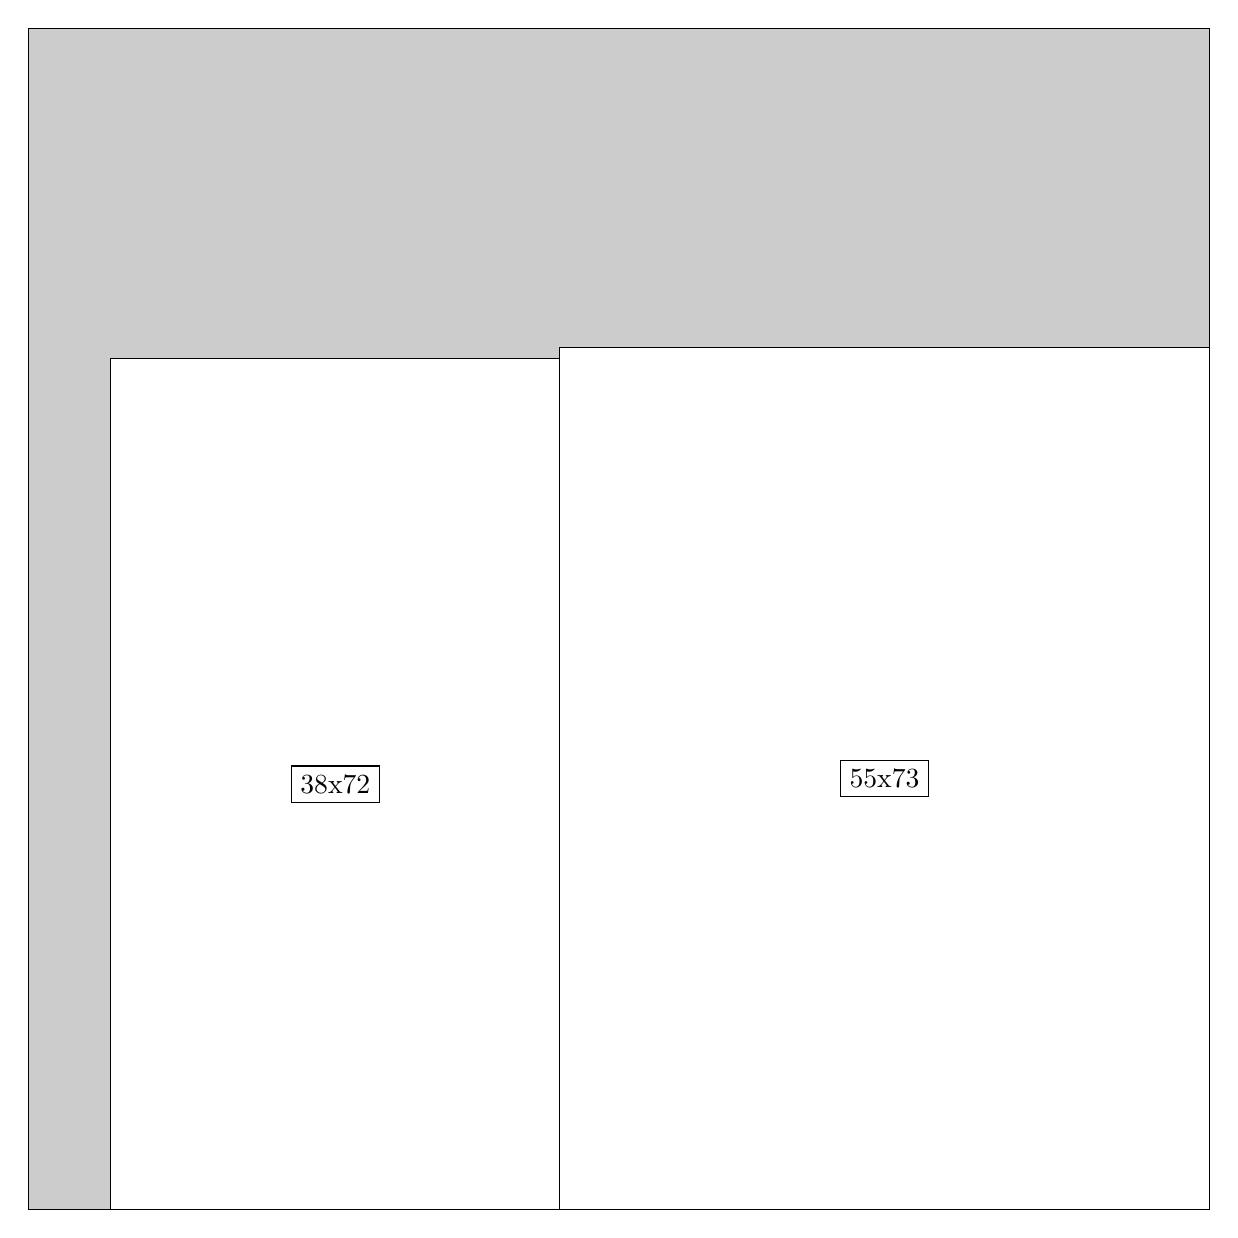
\begin{tikzpicture}[shorten >=1pt,scale=1.0,every node/.style={scale=1.0},->]
\tikzstyle{vertex}=[circle,fill=black!25,minimum size=14pt,inner sep=0pt]
\filldraw[fill=gray!40!white, draw=black] (0,0) rectangle (15.0,15.0);
\foreach \name/\x/\y/\w/\h in {55x73/6.75/0.0/8.25/10.95,38x72/1.05/0.0/5.7/10.799999999999999}
\filldraw[fill=white!40!white, draw=black] (\x,\y) rectangle node[draw] (\name) {\name} ++(\w,\h);
\end{tikzpicture}


w =55 , h =73 , x =45 , y =0 , v =4015
\par
w =38 , h =72 , x =7 , y =0 , v =2736
\par
\newpage


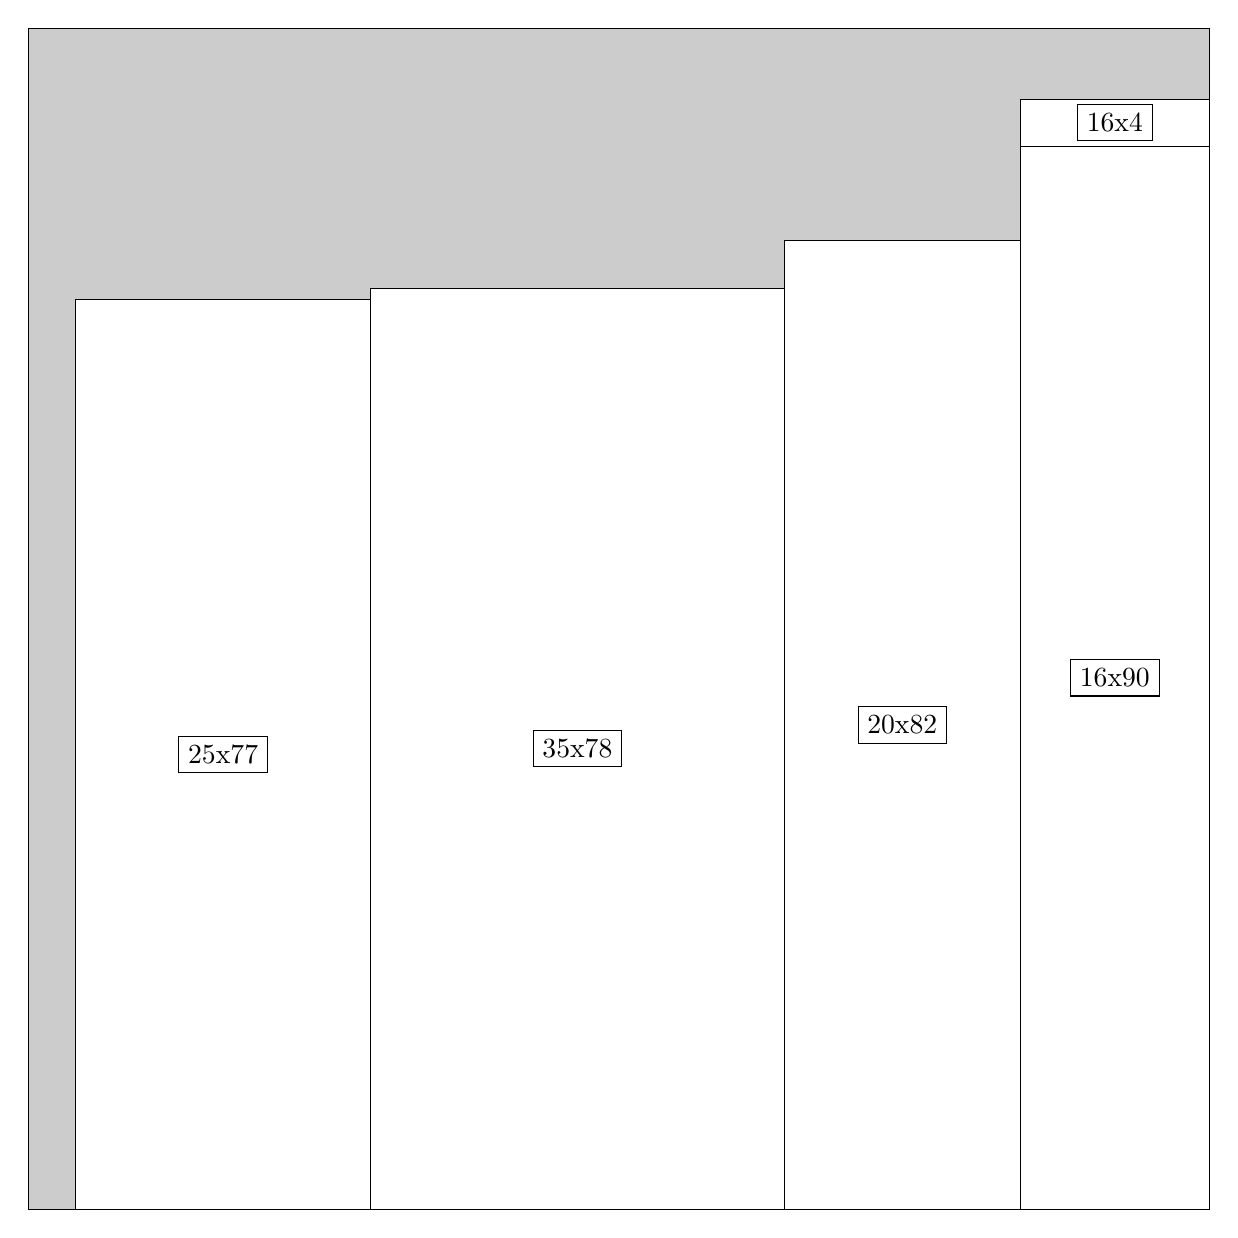
\begin{tikzpicture}[shorten >=1pt,scale=1.0,every node/.style={scale=1.0},->]
\tikzstyle{vertex}=[circle,fill=black!25,minimum size=14pt,inner sep=0pt]
\filldraw[fill=gray!40!white, draw=black] (0,0) rectangle (15.0,15.0);
\foreach \name/\x/\y/\w/\h in {16x90/12.6/0.0/2.4/13.5,16x4/12.6/13.5/2.4/0.6,20x82/9.6/0.0/3.0/12.299999999999999,35x78/4.35/0.0/5.25/11.7,25x77/0.6/0.0/3.75/11.549999999999999}
\filldraw[fill=white!40!white, draw=black] (\x,\y) rectangle node[draw] (\name) {\name} ++(\w,\h);
\end{tikzpicture}


w =16 , h =90 , x =84 , y =0 , v =1440
\par
w =16 , h =4 , x =84 , y =90 , v =64
\par
w =20 , h =82 , x =64 , y =0 , v =1640
\par
w =35 , h =78 , x =29 , y =0 , v =2730
\par
w =25 , h =77 , x =4 , y =0 , v =1925
\par
\newpage


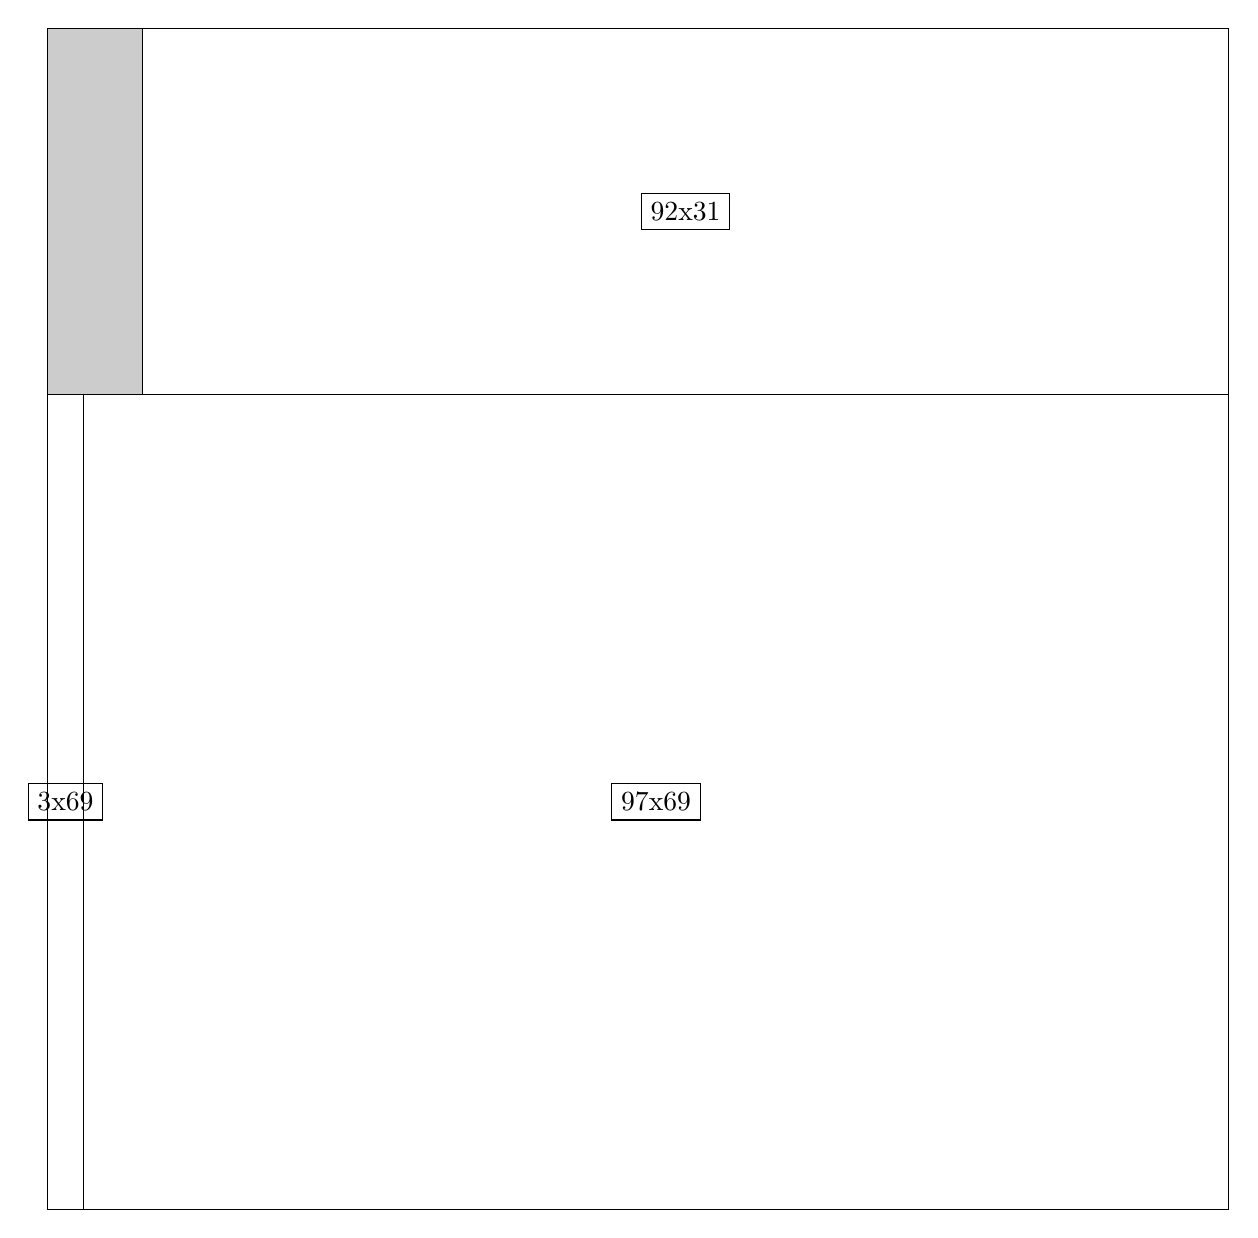
\begin{tikzpicture}[shorten >=1pt,scale=1.0,every node/.style={scale=1.0},->]
\tikzstyle{vertex}=[circle,fill=black!25,minimum size=14pt,inner sep=0pt]
\filldraw[fill=gray!40!white, draw=black] (0,0) rectangle (15.0,15.0);
\foreach \name/\x/\y/\w/\h in {97x69/0.44999999999999996/0.0/14.549999999999999/10.35,3x69/0.0/0.0/0.44999999999999996/10.35,92x31/1.2/10.35/13.799999999999999/4.6499999999999995}
\filldraw[fill=white!40!white, draw=black] (\x,\y) rectangle node[draw] (\name) {\name} ++(\w,\h);
\end{tikzpicture}


w =97 , h =69 , x =3 , y =0 , v =6693
\par
w =3 , h =69 , x =0 , y =0 , v =207
\par
w =92 , h =31 , x =8 , y =69 , v =2852
\par
\newpage


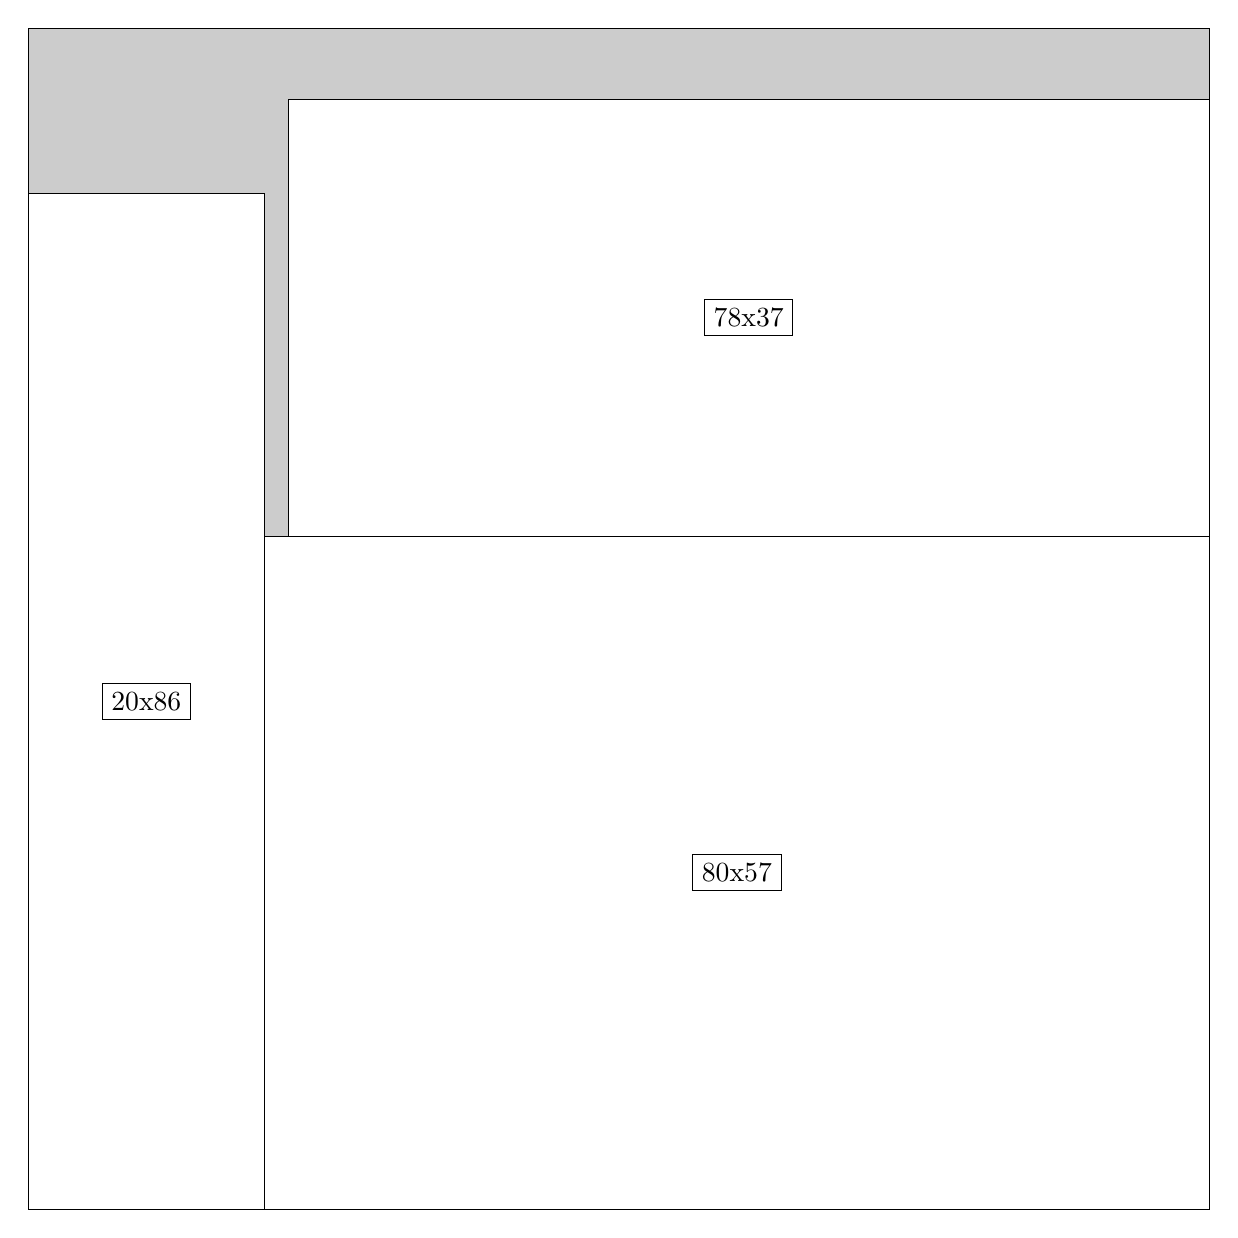
\begin{tikzpicture}[shorten >=1pt,scale=1.0,every node/.style={scale=1.0},->]
\tikzstyle{vertex}=[circle,fill=black!25,minimum size=14pt,inner sep=0pt]
\filldraw[fill=gray!40!white, draw=black] (0,0) rectangle (15.0,15.0);
\foreach \name/\x/\y/\w/\h in {80x57/3.0/0.0/12.0/8.549999999999999,78x37/3.3/8.549999999999999/11.7/5.55,20x86/0.0/0.0/3.0/12.9}
\filldraw[fill=white!40!white, draw=black] (\x,\y) rectangle node[draw] (\name) {\name} ++(\w,\h);
\end{tikzpicture}


w =80 , h =57 , x =20 , y =0 , v =4560
\par
w =78 , h =37 , x =22 , y =57 , v =2886
\par
w =20 , h =86 , x =0 , y =0 , v =1720
\par
\newpage


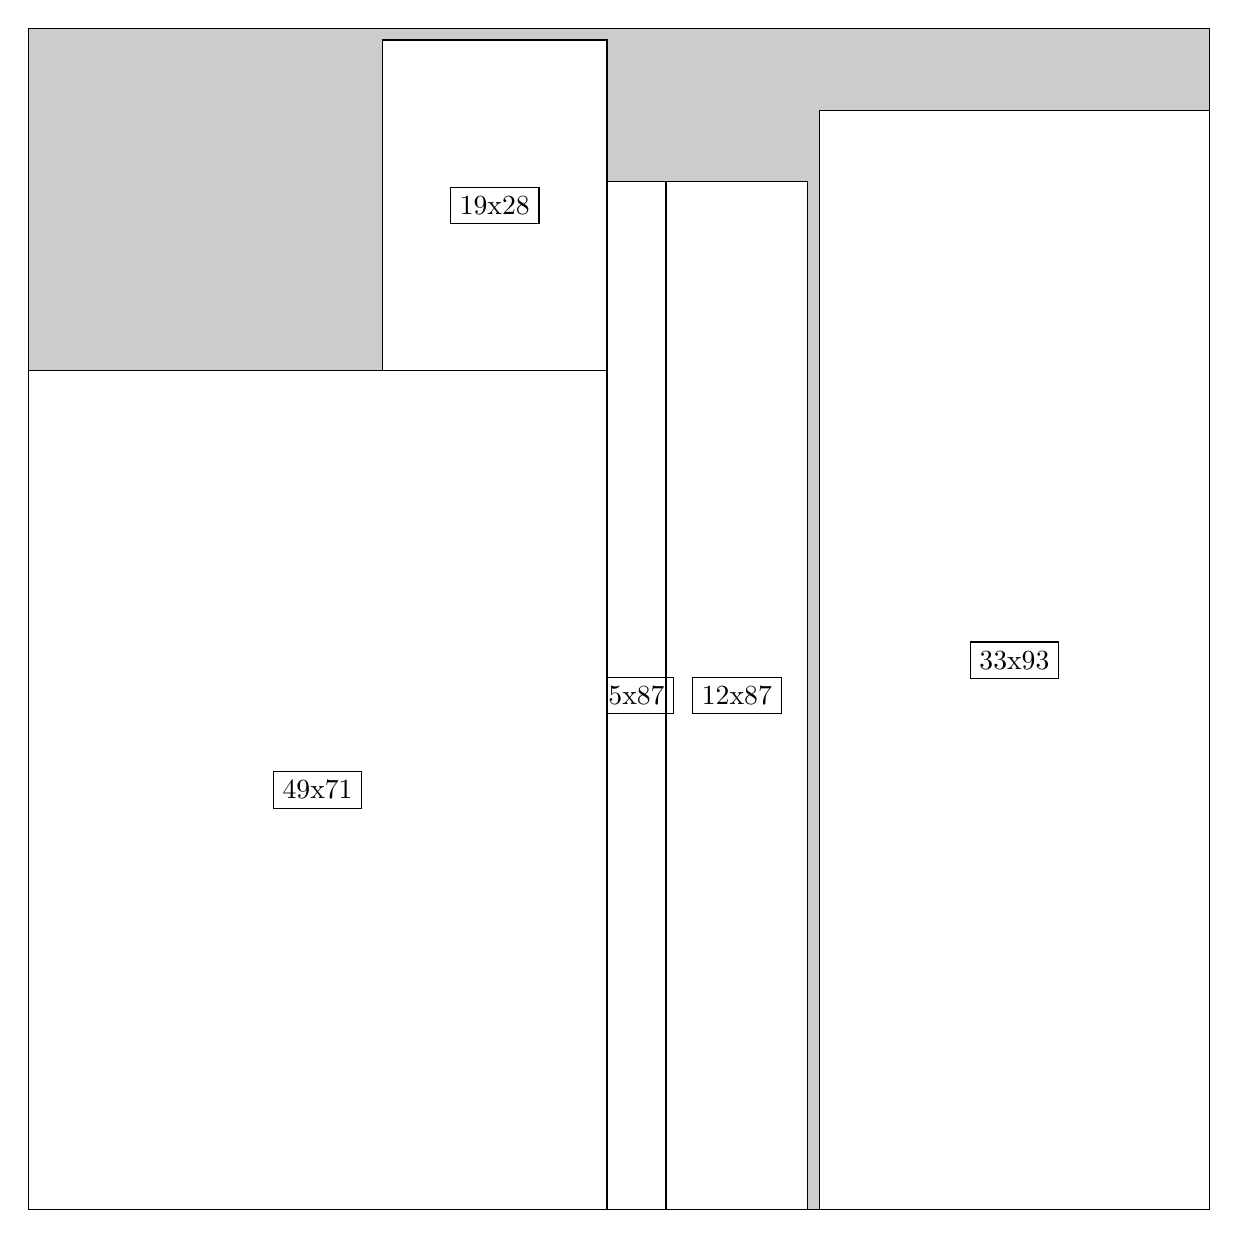
\begin{tikzpicture}[shorten >=1pt,scale=1.0,every node/.style={scale=1.0},->]
\tikzstyle{vertex}=[circle,fill=black!25,minimum size=14pt,inner sep=0pt]
\filldraw[fill=gray!40!white, draw=black] (0,0) rectangle (15.0,15.0);
\foreach \name/\x/\y/\w/\h in {33x93/10.049999999999999/0.0/4.95/13.95,12x87/8.1/0.0/1.7999999999999998/13.049999999999999,5x87/7.35/0.0/0.75/13.049999999999999,49x71/0.0/0.0/7.35/10.65,19x28/4.5/10.65/2.85/4.2}
\filldraw[fill=white!40!white, draw=black] (\x,\y) rectangle node[draw] (\name) {\name} ++(\w,\h);
\end{tikzpicture}


w =33 , h =93 , x =67 , y =0 , v =3069
\par
w =12 , h =87 , x =54 , y =0 , v =1044
\par
w =5 , h =87 , x =49 , y =0 , v =435
\par
w =49 , h =71 , x =0 , y =0 , v =3479
\par
w =19 , h =28 , x =30 , y =71 , v =532
\par
\newpage


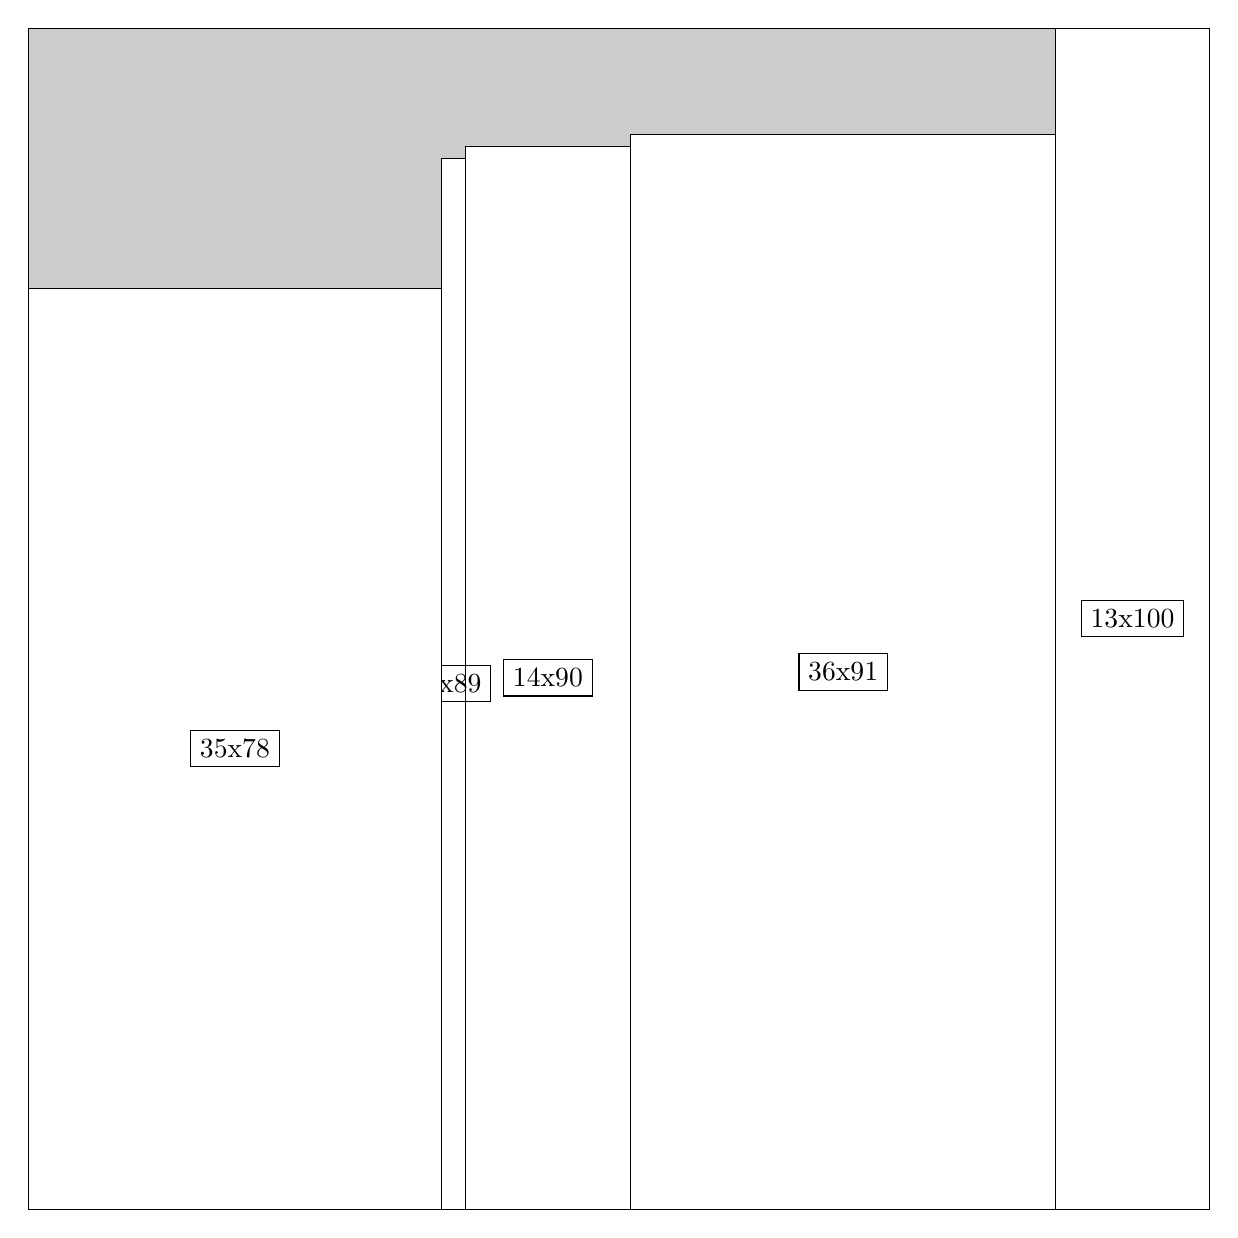
\begin{tikzpicture}[shorten >=1pt,scale=1.0,every node/.style={scale=1.0},->]
\tikzstyle{vertex}=[circle,fill=black!25,minimum size=14pt,inner sep=0pt]
\filldraw[fill=gray!40!white, draw=black] (0,0) rectangle (15.0,15.0);
\foreach \name/\x/\y/\w/\h in {13x100/13.049999999999999/0.0/1.95/15.0,36x91/7.6499999999999995/0.0/5.3999999999999995/13.65,14x90/5.55/0.0/2.1/13.5,2x89/5.25/0.0/0.3/13.35,35x78/0.0/0.0/5.25/11.7}
\filldraw[fill=white!40!white, draw=black] (\x,\y) rectangle node[draw] (\name) {\name} ++(\w,\h);
\end{tikzpicture}


w =13 , h =100 , x =87 , y =0 , v =1300
\par
w =36 , h =91 , x =51 , y =0 , v =3276
\par
w =14 , h =90 , x =37 , y =0 , v =1260
\par
w =2 , h =89 , x =35 , y =0 , v =178
\par
w =35 , h =78 , x =0 , y =0 , v =2730
\par
\newpage


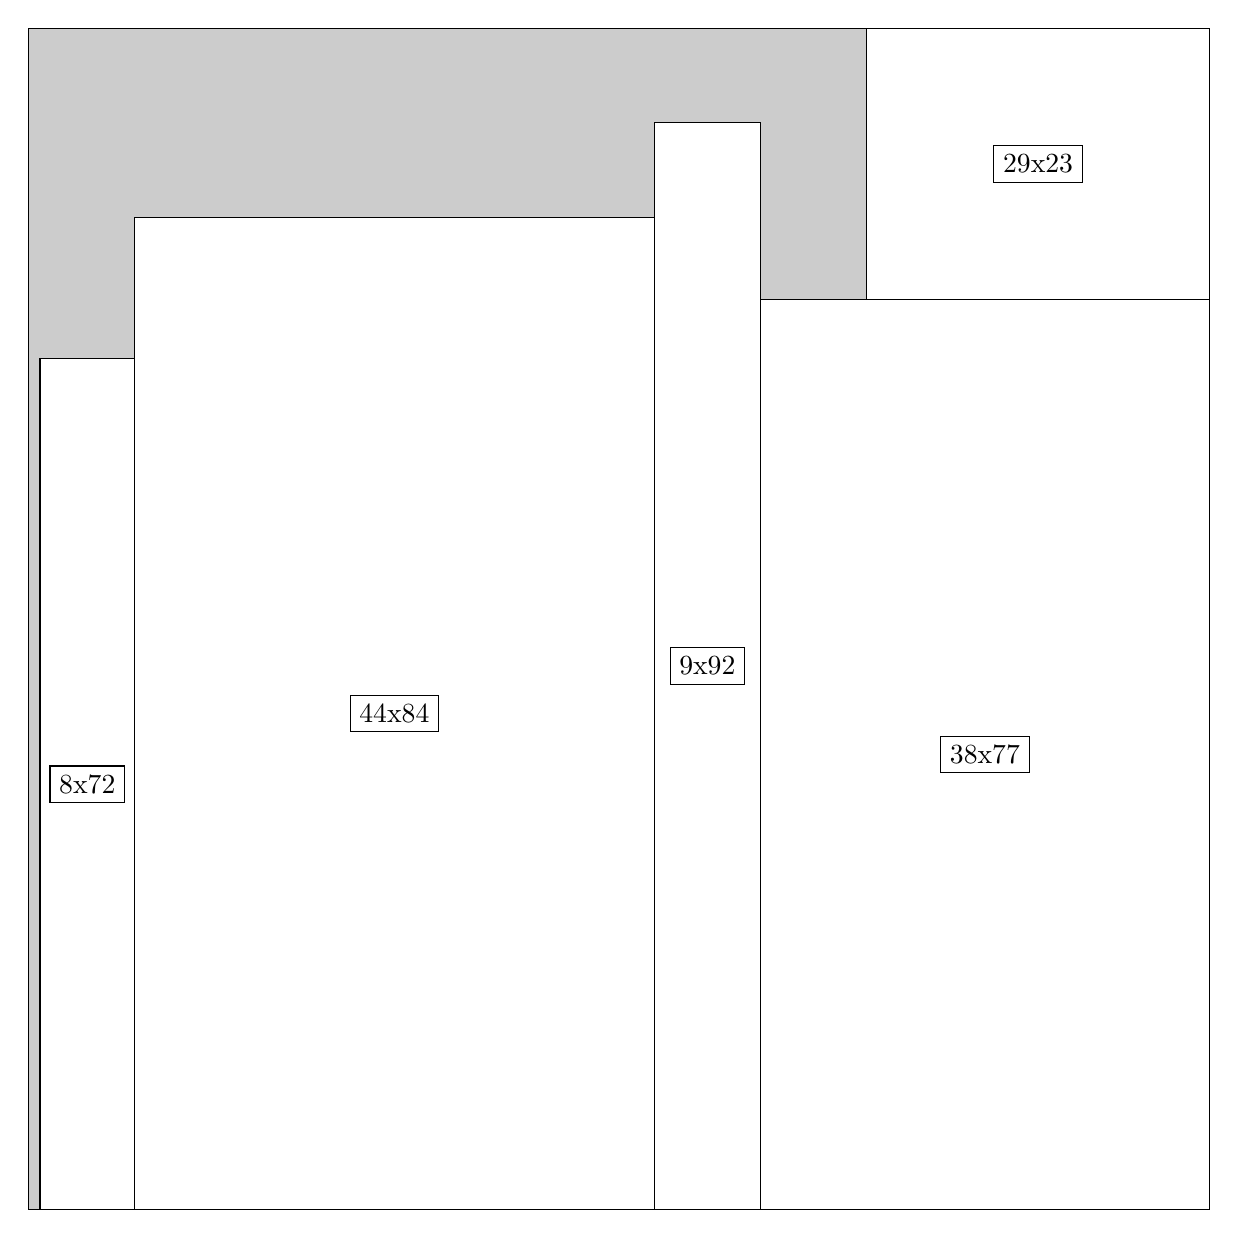
\begin{tikzpicture}[shorten >=1pt,scale=1.0,every node/.style={scale=1.0},->]
\tikzstyle{vertex}=[circle,fill=black!25,minimum size=14pt,inner sep=0pt]
\filldraw[fill=gray!40!white, draw=black] (0,0) rectangle (15.0,15.0);
\foreach \name/\x/\y/\w/\h in {38x77/9.299999999999999/0.0/5.7/11.549999999999999,29x23/10.65/11.549999999999999/4.35/3.4499999999999997,9x92/7.949999999999999/0.0/1.3499999999999999/13.799999999999999,44x84/1.3499999999999999/0.0/6.6/12.6,8x72/0.15/0.0/1.2/10.799999999999999}
\filldraw[fill=white!40!white, draw=black] (\x,\y) rectangle node[draw] (\name) {\name} ++(\w,\h);
\end{tikzpicture}


w =38 , h =77 , x =62 , y =0 , v =2926
\par
w =29 , h =23 , x =71 , y =77 , v =667
\par
w =9 , h =92 , x =53 , y =0 , v =828
\par
w =44 , h =84 , x =9 , y =0 , v =3696
\par
w =8 , h =72 , x =1 , y =0 , v =576
\par
\newpage


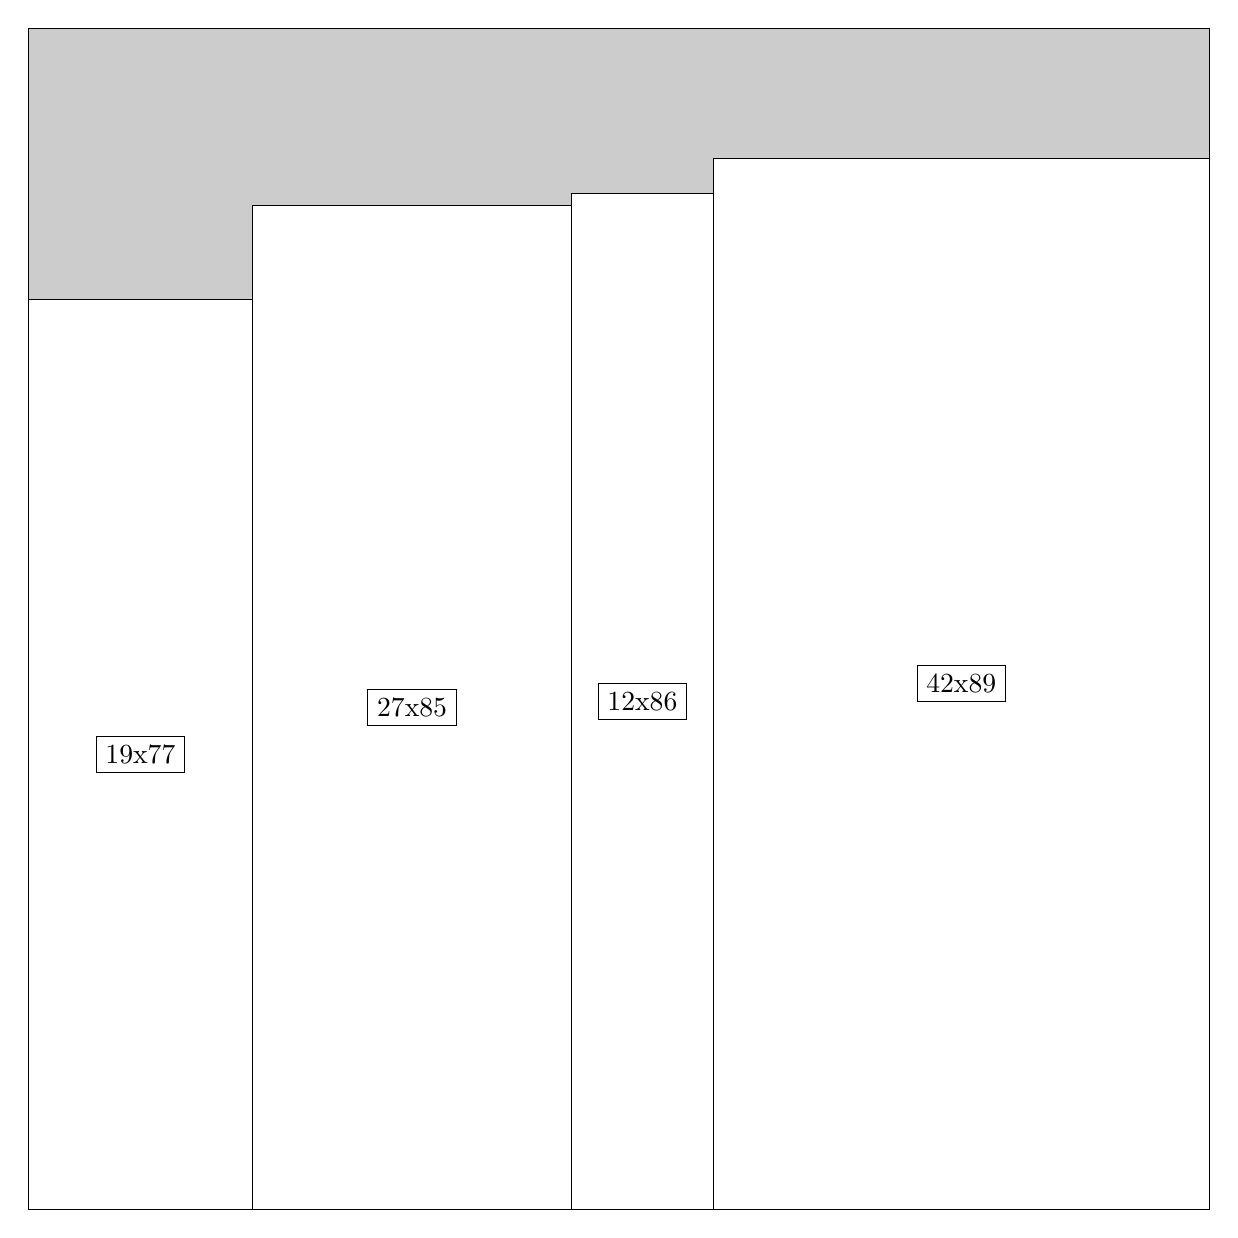
\begin{tikzpicture}[shorten >=1pt,scale=1.0,every node/.style={scale=1.0},->]
\tikzstyle{vertex}=[circle,fill=black!25,minimum size=14pt,inner sep=0pt]
\filldraw[fill=gray!40!white, draw=black] (0,0) rectangle (15.0,15.0);
\foreach \name/\x/\y/\w/\h in {42x89/8.7/0.0/6.3/13.35,12x86/6.8999999999999995/0.0/1.7999999999999998/12.9,27x85/2.85/0.0/4.05/12.75,19x77/0.0/0.0/2.85/11.549999999999999}
\filldraw[fill=white!40!white, draw=black] (\x,\y) rectangle node[draw] (\name) {\name} ++(\w,\h);
\end{tikzpicture}


w =42 , h =89 , x =58 , y =0 , v =3738
\par
w =12 , h =86 , x =46 , y =0 , v =1032
\par
w =27 , h =85 , x =19 , y =0 , v =2295
\par
w =19 , h =77 , x =0 , y =0 , v =1463
\par
\newpage


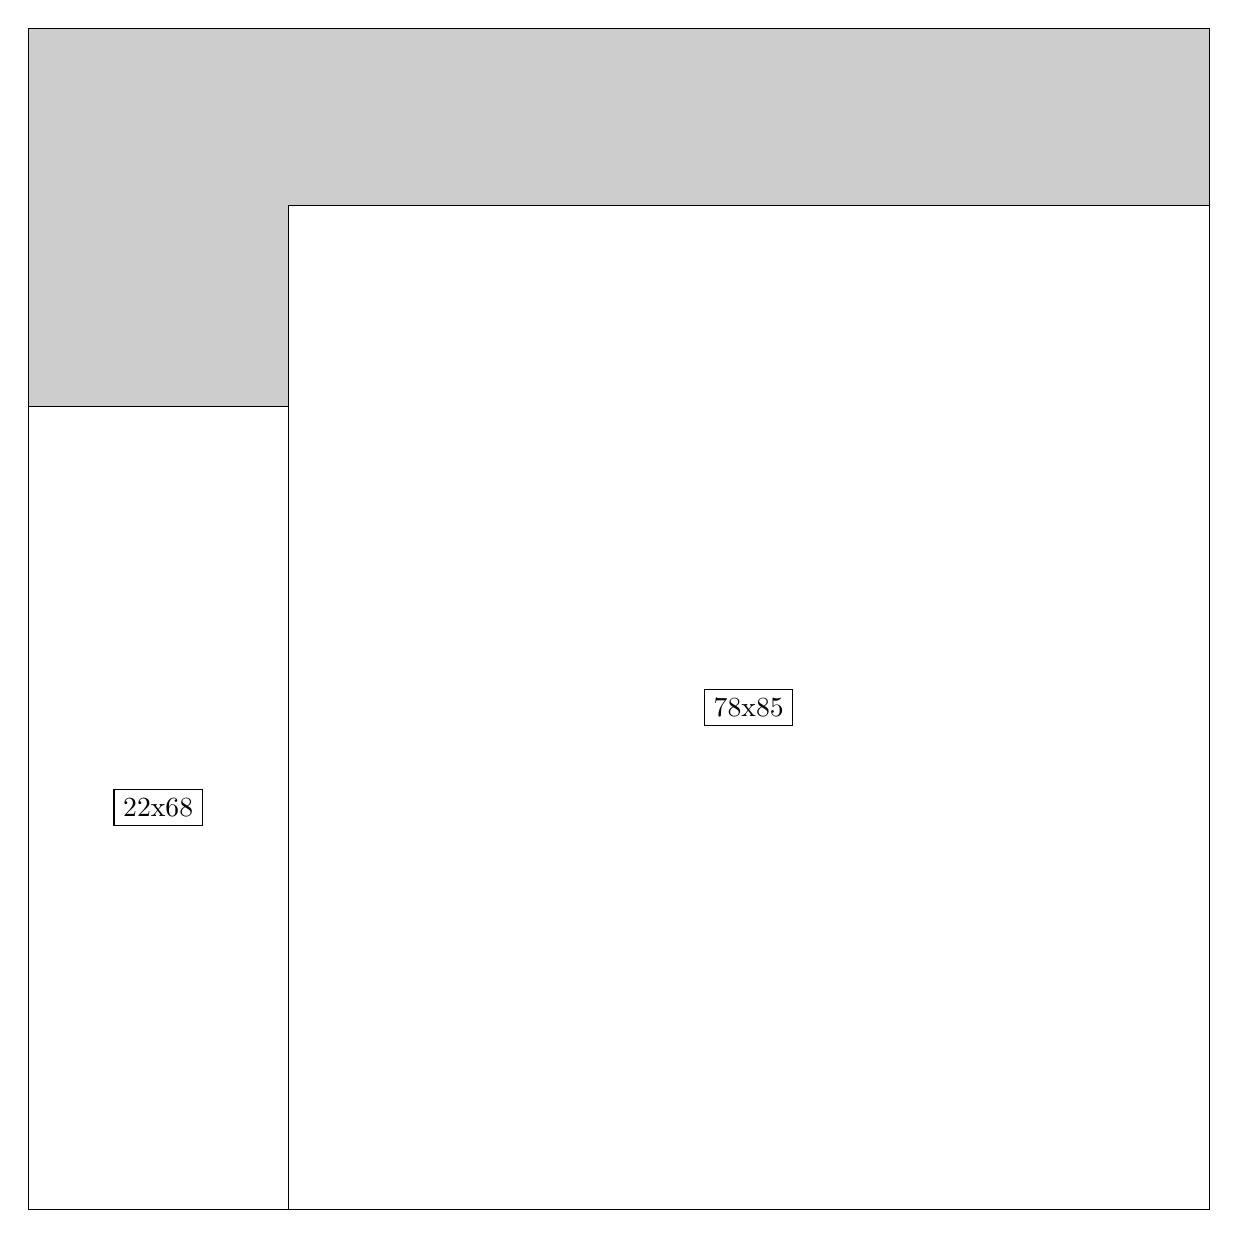
\begin{tikzpicture}[shorten >=1pt,scale=1.0,every node/.style={scale=1.0},->]
\tikzstyle{vertex}=[circle,fill=black!25,minimum size=14pt,inner sep=0pt]
\filldraw[fill=gray!40!white, draw=black] (0,0) rectangle (15.0,15.0);
\foreach \name/\x/\y/\w/\h in {78x85/3.3/0.0/11.7/12.75,22x68/0.0/0.0/3.3/10.2}
\filldraw[fill=white!40!white, draw=black] (\x,\y) rectangle node[draw] (\name) {\name} ++(\w,\h);
\end{tikzpicture}


w =78 , h =85 , x =22 , y =0 , v =6630
\par
w =22 , h =68 , x =0 , y =0 , v =1496
\par
\newpage


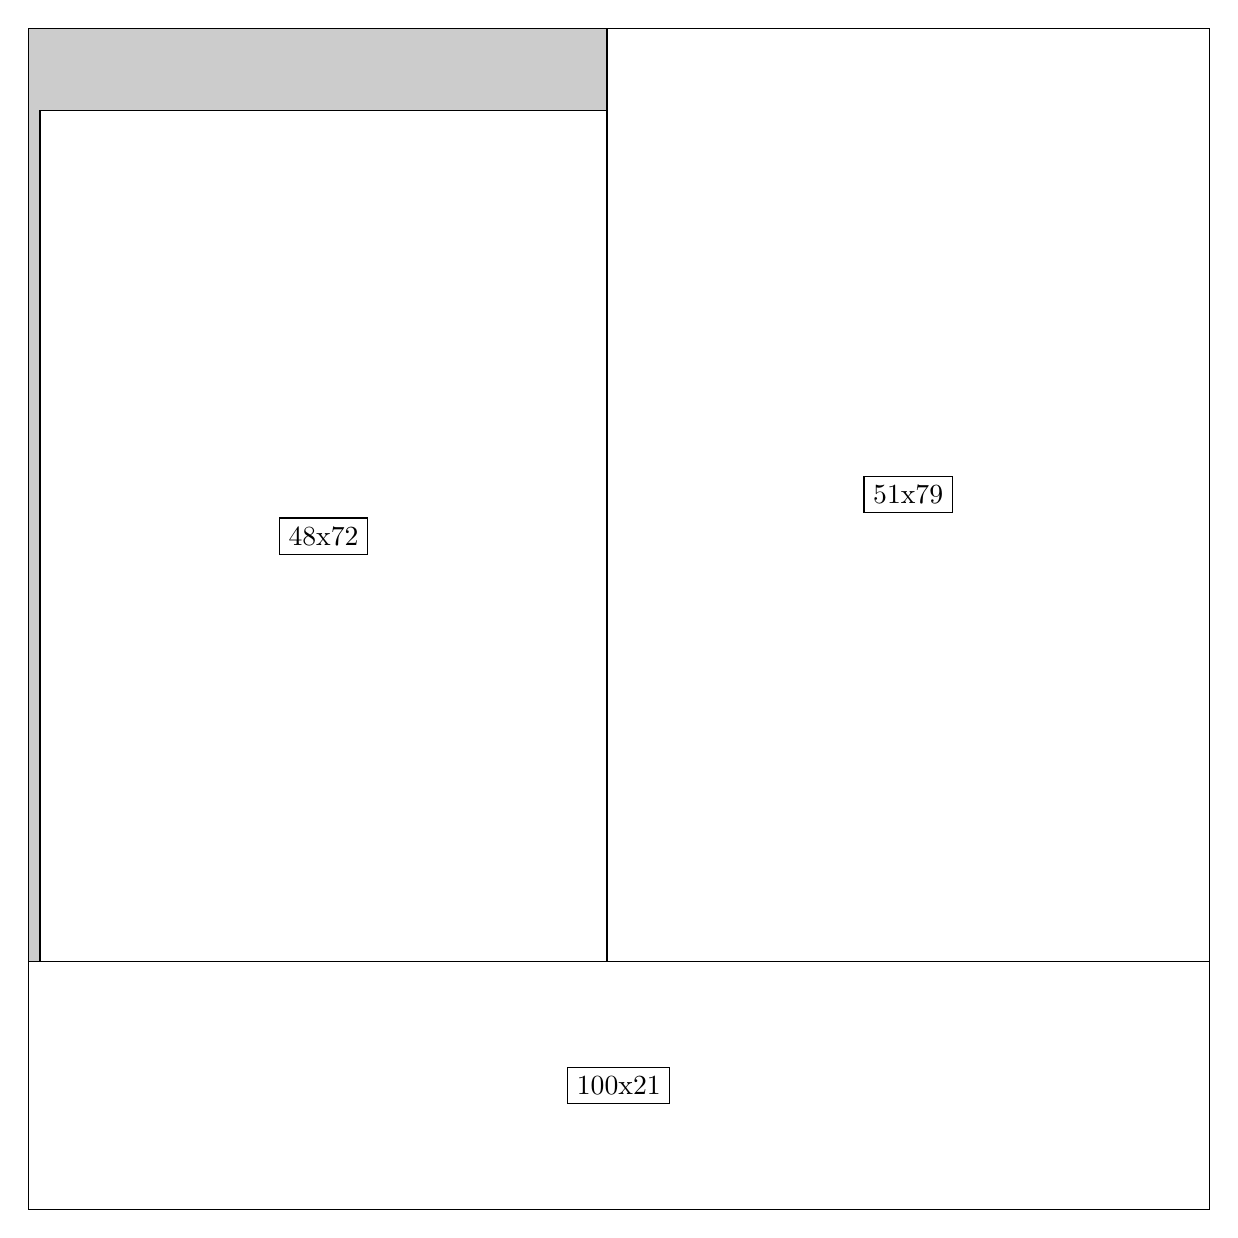
\begin{tikzpicture}[shorten >=1pt,scale=1.0,every node/.style={scale=1.0},->]
\tikzstyle{vertex}=[circle,fill=black!25,minimum size=14pt,inner sep=0pt]
\filldraw[fill=gray!40!white, draw=black] (0,0) rectangle (15.0,15.0);
\foreach \name/\x/\y/\w/\h in {100x21/0.0/0.0/15.0/3.15,51x79/7.35/3.15/7.6499999999999995/11.85,48x72/0.15/3.15/7.199999999999999/10.799999999999999}
\filldraw[fill=white!40!white, draw=black] (\x,\y) rectangle node[draw] (\name) {\name} ++(\w,\h);
\end{tikzpicture}


w =100 , h =21 , x =0 , y =0 , v =2100
\par
w =51 , h =79 , x =49 , y =21 , v =4029
\par
w =48 , h =72 , x =1 , y =21 , v =3456
\par
\newpage


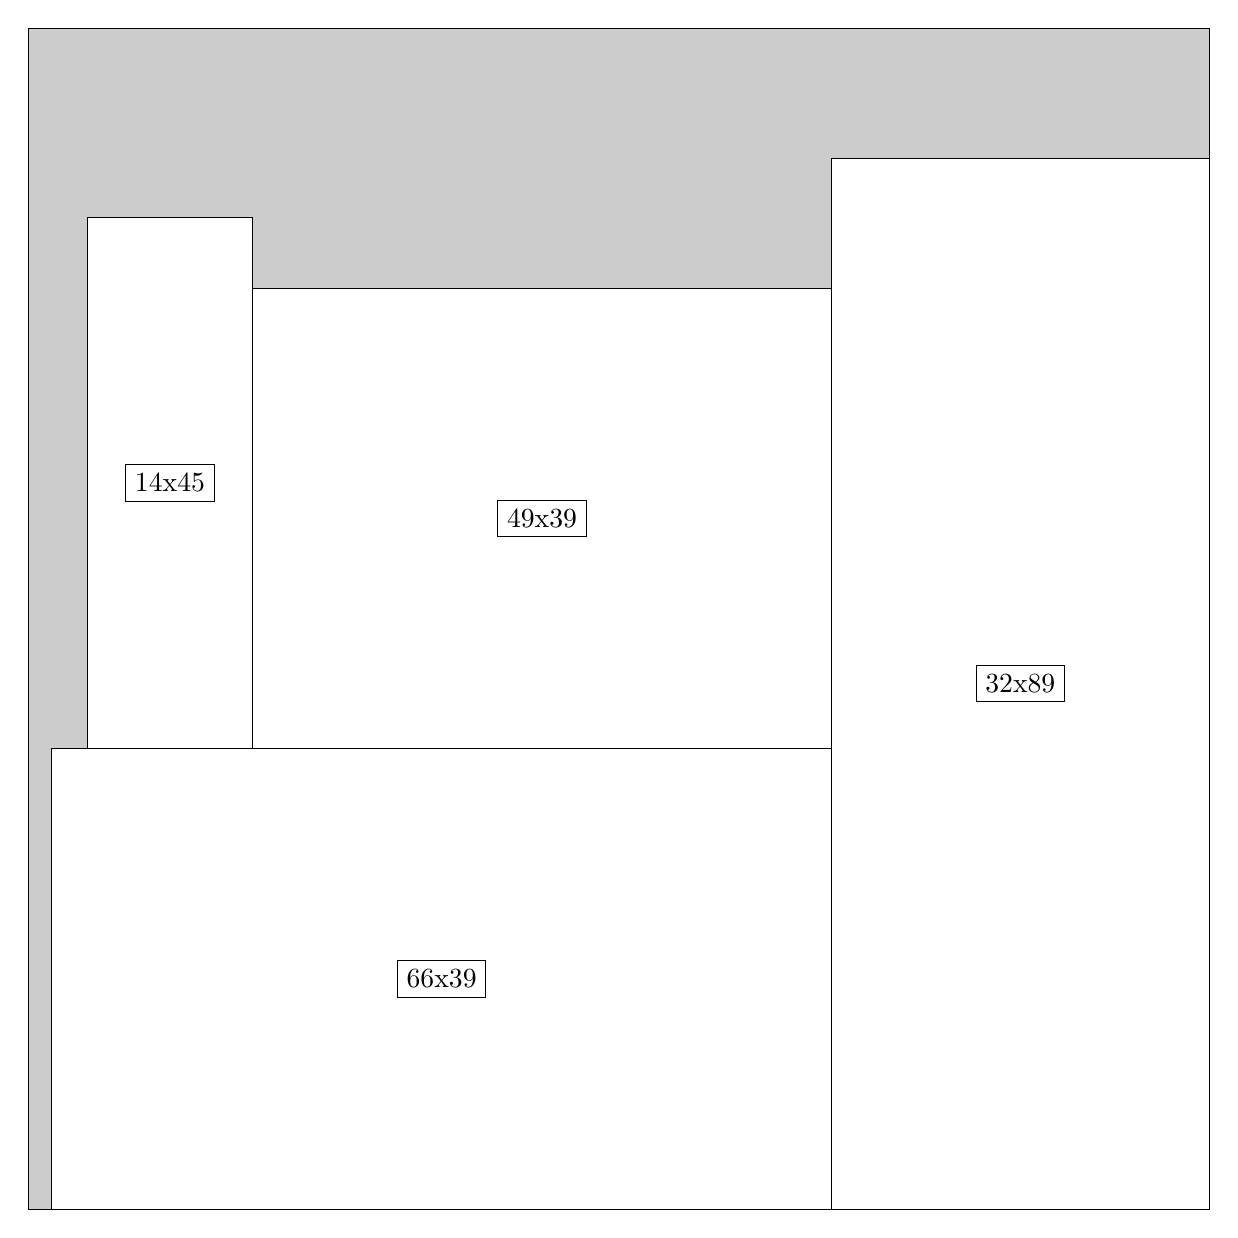
\begin{tikzpicture}[shorten >=1pt,scale=1.0,every node/.style={scale=1.0},->]
\tikzstyle{vertex}=[circle,fill=black!25,minimum size=14pt,inner sep=0pt]
\filldraw[fill=gray!40!white, draw=black] (0,0) rectangle (15.0,15.0);
\foreach \name/\x/\y/\w/\h in {32x89/10.2/0.0/4.8/13.35,66x39/0.3/0.0/9.9/5.85,49x39/2.85/5.85/7.35/5.85,14x45/0.75/5.85/2.1/6.75}
\filldraw[fill=white!40!white, draw=black] (\x,\y) rectangle node[draw] (\name) {\name} ++(\w,\h);
\end{tikzpicture}


w =32 , h =89 , x =68 , y =0 , v =2848
\par
w =66 , h =39 , x =2 , y =0 , v =2574
\par
w =49 , h =39 , x =19 , y =39 , v =1911
\par
w =14 , h =45 , x =5 , y =39 , v =630
\par
\newpage


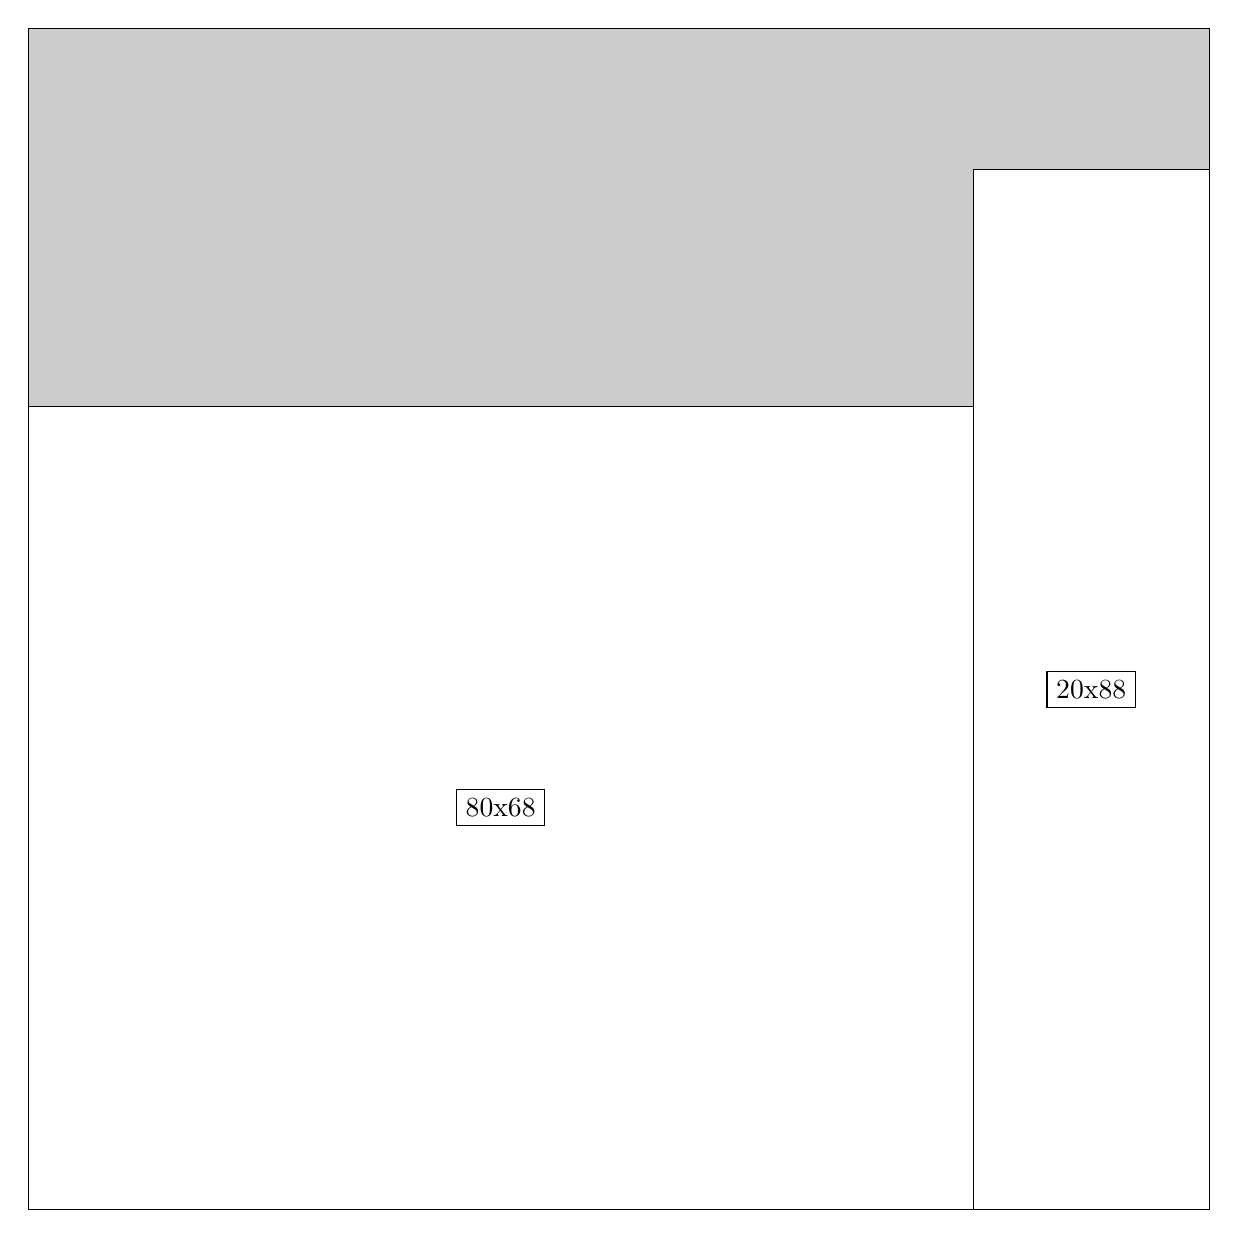
\begin{tikzpicture}[shorten >=1pt,scale=1.0,every node/.style={scale=1.0},->]
\tikzstyle{vertex}=[circle,fill=black!25,minimum size=14pt,inner sep=0pt]
\filldraw[fill=gray!40!white, draw=black] (0,0) rectangle (15.0,15.0);
\foreach \name/\x/\y/\w/\h in {20x88/12.0/0.0/3.0/13.2,80x68/0.0/0.0/12.0/10.2}
\filldraw[fill=white!40!white, draw=black] (\x,\y) rectangle node[draw] (\name) {\name} ++(\w,\h);
\end{tikzpicture}


w =20 , h =88 , x =80 , y =0 , v =1760
\par
w =80 , h =68 , x =0 , y =0 , v =5440
\par
\newpage


\end{document}